%A child has a die whose six faces show the letters as given below:\\

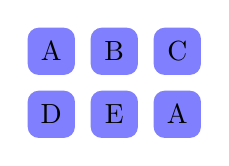
\begin{tikzpicture}[outer sep=0.05cm,node distance=0.8cm,]
\tikzstyle{bigbox} = [draw=white!50, thick, fill=white!10, rounded corners, rectangle]
\tikzstyle{box} = [minimum size=0.6cm, rounded corners,rectangle, fill=blue!50]
%
\node[box] (11) {A};
\node[box,right of=11] (12) {B};
\node[box,right of=12] (13) {C};
\node[box,below of=11] (21) {D};
\node[box,right of=21] (22) {E};
\node[box,right of=22] (23) {A};
\end{tikzpicture}
%\\
%The die is thrown once. What is the probability of getting (i) A? (ii) D?
